\documentclass[12pt,letterpaper]{article}
%\usepackage{fullpage}
\usepackage[top=2cm, bottom=4.5cm, left=2.5cm, right=2.5cm]{geometry}
\usepackage{amsmath,amsthm,amsfonts,amssymb,amscd}
%\usepackage{lastpage}
\usepackage{enumerate}
\usepackage{fancyhdr}
%\usepackage{mathrsfs}
\usepackage{xcolor}
\usepackage{graphicx}
\usepackage{listings}
\usepackage{hyperref}

\hypersetup{%
  colorlinks=true,
  linkcolor=blue,
  linkbordercolor={0 0 1}
}
 
\renewcommand\lstlistingname{Algorithm}
\renewcommand\lstlistlistingname{Algorithms}
\def\lstlistingautorefname{Alg.}

\lstdefinestyle{Python}{
    language        = Python,
    frame           = lines, 
    basicstyle      = \footnotesize,
    keywordstyle    = \color{blue},
    stringstyle     = \color{green},
    commentstyle    = \color{red}\ttfamily
}

\setlength{\parindent}{0.0in}
\setlength{\parskip}{0.05in}

% Edit these as appropriate

\pagestyle{fancyplain}
\headheight 35pt
\lhead{Shriram R \\ 06-02-01-10-51-18-1-15763} 
\chead{\textbf{\Large Assignment 0}}
\rhead{DS 211 \\ Due: Aug 16, 2019}
\lfoot{}
\cfoot{}
\rfoot{\small\thepage}
\headsep 1.5em

\begin{document}

\section*{Problem 1}

\begin{enumerate}
  \item
   The derivative $f'(x) = \frac{-12x}{(6x^2-1)^2}$.
  \item
   $f(0.408) = \infty $ (denominator became $0$) using 3-digit arithmetic and $f(0.408) = 833.3$ using 4-digit arithmetic with rounding.
  \item
  Horner's representation of the given polynomial is $y = -0.35 + x(8 + x(-7 + x))$. The value of $y$ at $x=1.37$ is $0.048$ using 3-digit arithmetic rounding.
  \item 
  The value of $y$ at $x=1.37$ is $0.02$ using direct substitution and 3-digit arithmetic rounding.
  \item 
  The value computed using Horner's rule is more accurate since it is closer the actual value without rounding which is $0.0431$.  
\end{enumerate}


\section*{Problem 2}

\begin{enumerate}
	\item The RAM size necessary to store the given array is $49439$ MB.
	\item No. $32$ GB is not sufficient to store the entire array in RAM alone. But swap space could be used to spill excess array to disk and still use the RAM.
	\item No. It is not possible to use the workstation as this increase in resolution requires $111^2$ more space than the previous array which amounts to roughly $600$ TB.	
\end{enumerate}

\section*{Problem 3}

\begin{enumerate}
	\item 
	\item 
	\item 
	\item 
	\item
\end{enumerate}

\section*{Problem 4}

\begin{enumerate}
	\item The functions have been implemented in scgs.m and smgs.m files.
	\item Matrix generation function has been implemented in matgen.m file.
	\item The script to run for different matrix sizes is written in exp.m file.
	\item The plot for error is available below,
	\begin{figure}[!h]
		\centering
		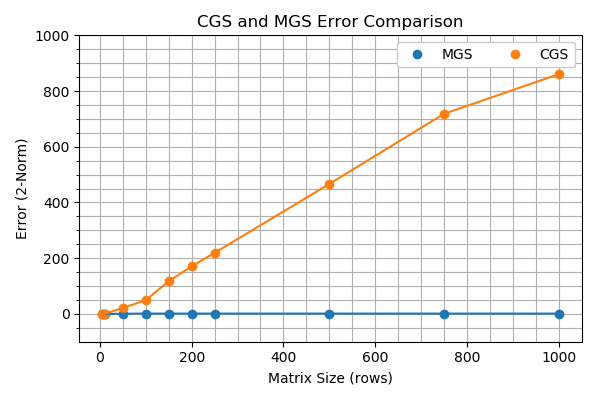
\includegraphics[width=0.9\linewidth]{1.png}
		\caption{CGS and MGS Error Comparison}
	\end{figure}
	\item The modified Gram-Schmidt technique is more numerically stable than the classical version. Error remains low and constant for modified technique and increases linearly with respect to matrix size for classical version.
\end{enumerate}

\section*{Problem 5}

   


\end{document}